Snímky vzorku 3 jsou na obrázcích \ref{o:vz3_01} a \ref{o:vz3_02}. Je zde patrný kompoziční kontrast.
Na obrázku \ref{o:vz3_body} jsou vyznačené body, ve kterých jsme prováděli kvantitativní analýzu RTG spektra. Výsledky jsou v tabulkách \ref{t:vz03_X}, \ref{t:vz03_Y}, \ref{t:vz03_Z} a obrázcích \ref{o:vz3_X}, \ref{o:vz3_Y}, \ref{o:vz3_Z}. Také jsme provedli lineární a 2D sken přechodu (obrázek \ref{o:vz3_2D})

\begin{figure}[htbp]
\centering
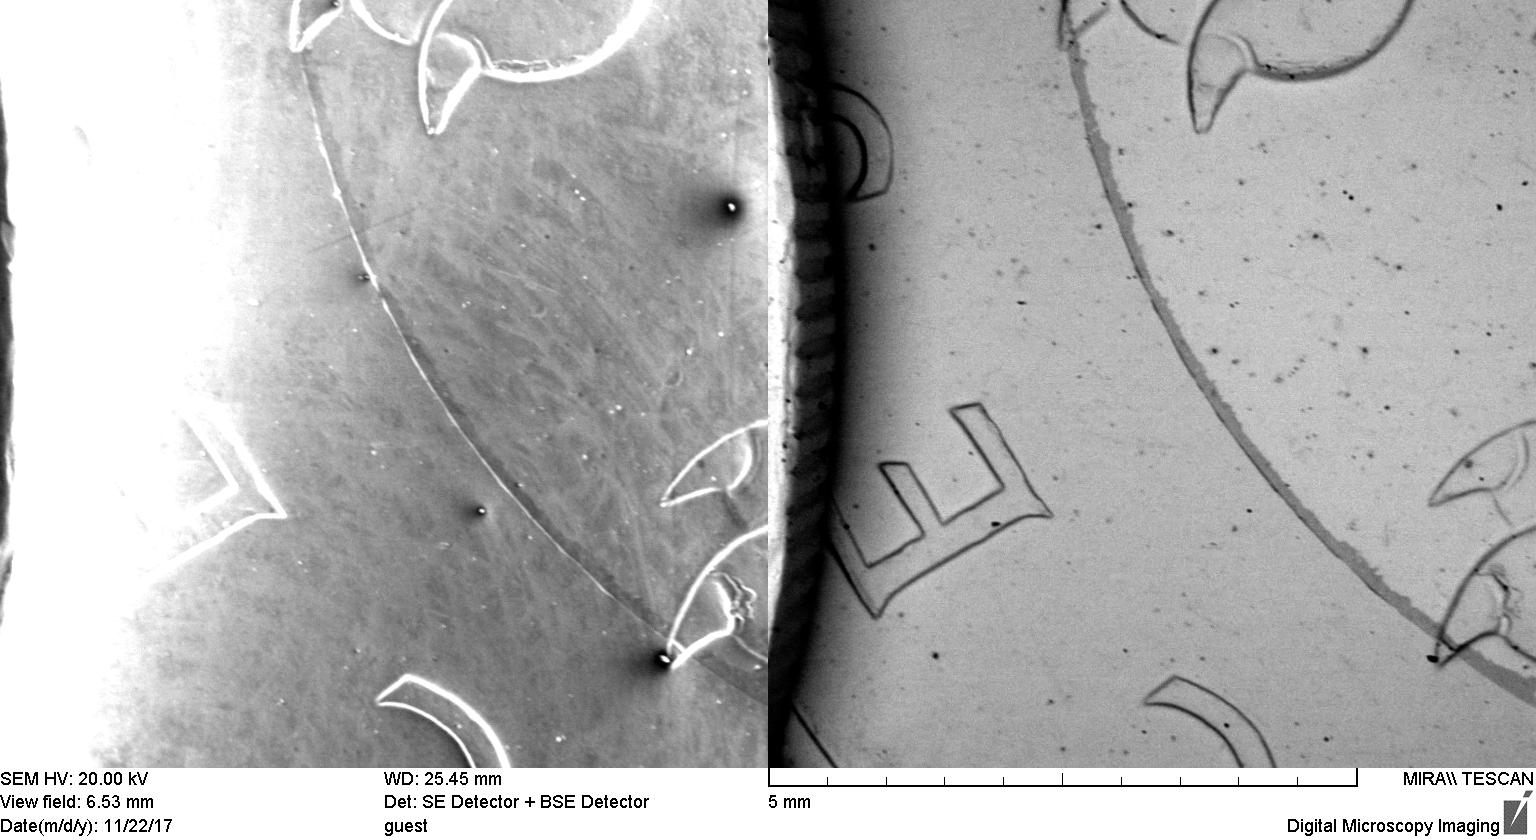
\includegraphics[width=\textwidth-2cm]{graficos/VZ03_01.png}
\caption{Vzorek 3}
\label{o:vz3_01}
\end{figure}

\begin{figure}[htbp]
\centering
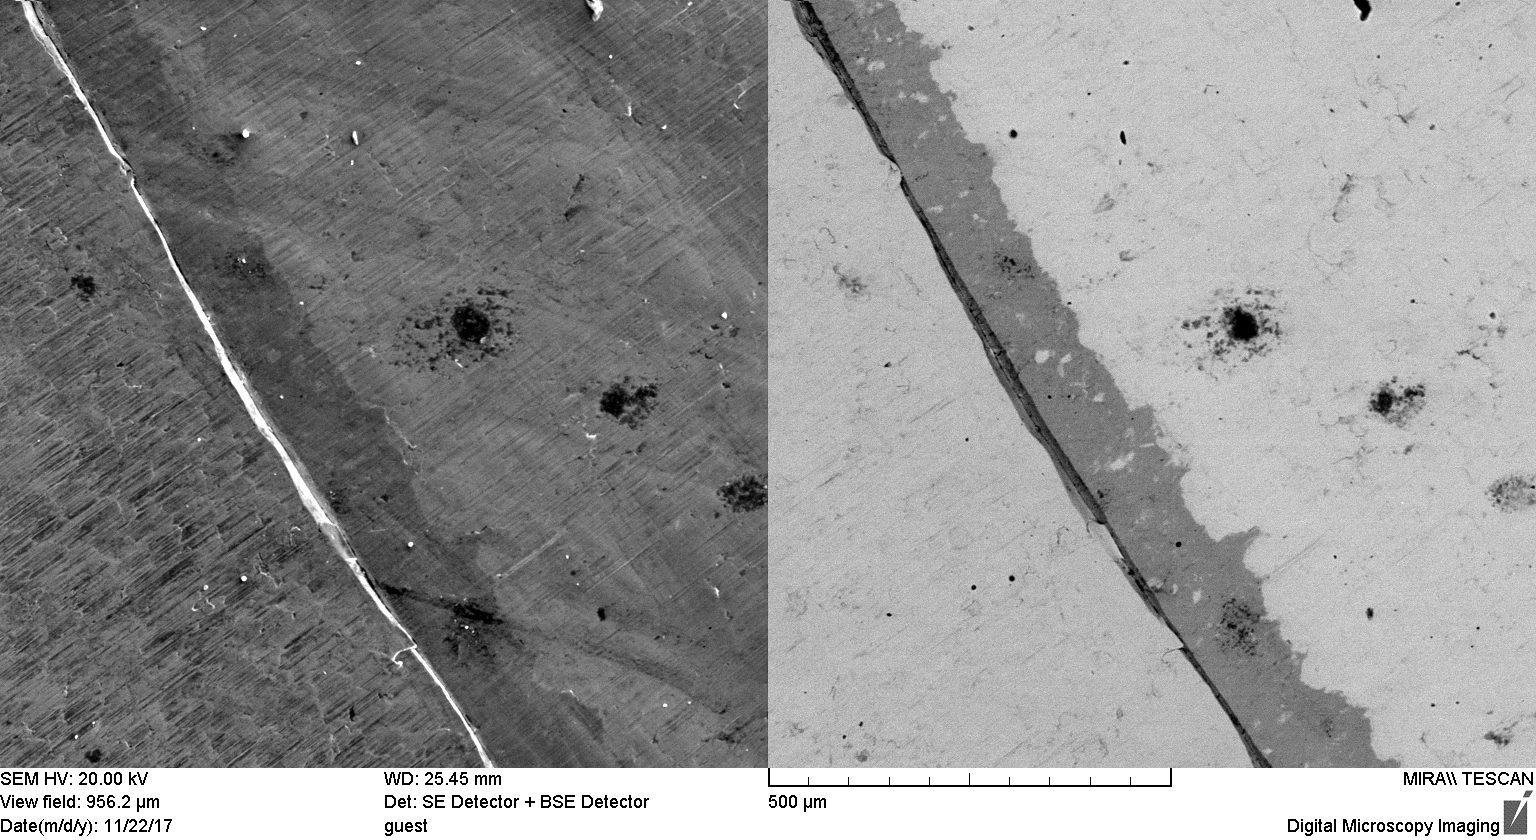
\includegraphics[width=\textwidth-2cm]{graficos/VZ03_02.png}
\caption{Vzorek 3}
\label{o:vz3_02}
\end{figure}

\begin{figure}[htbp]
\centering
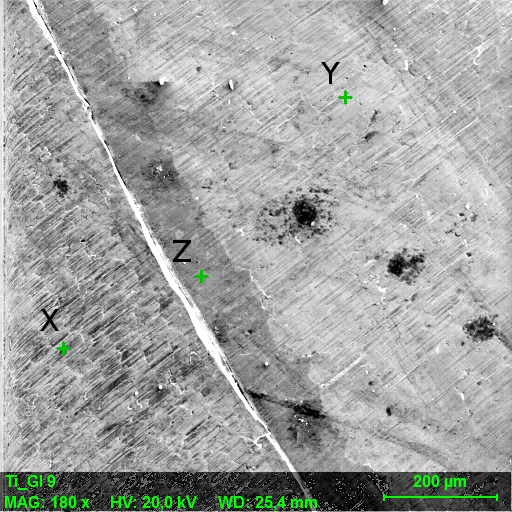
\includegraphics[width=8cm]{graficos/3/body.png}
\caption{Body, ve kterých jsme pozorovali RTG spektrum}
\label{o:vz3_body}
\end{figure}


\begin{tabulka}[htbp]
\centering
\begin{BVerbatim}
Spectrum: Ti_Gl_1 15

Element  Series   unn. C norm. C Atom. C Error
                 [wt.-%] [wt.-%] [at.-%]   [%]
----------------------------------------------
Copper  K-series   89,51  100,00  100,00   2,4
----------------------------------------------
          Total:   89,51  100,00  100,00
\end{BVerbatim}
\caption{Chemické složení vzorku 3 v místě X}
\label{t:vz03_X}
\end{tabulka}

\begin{figure}[htbp]
\centering
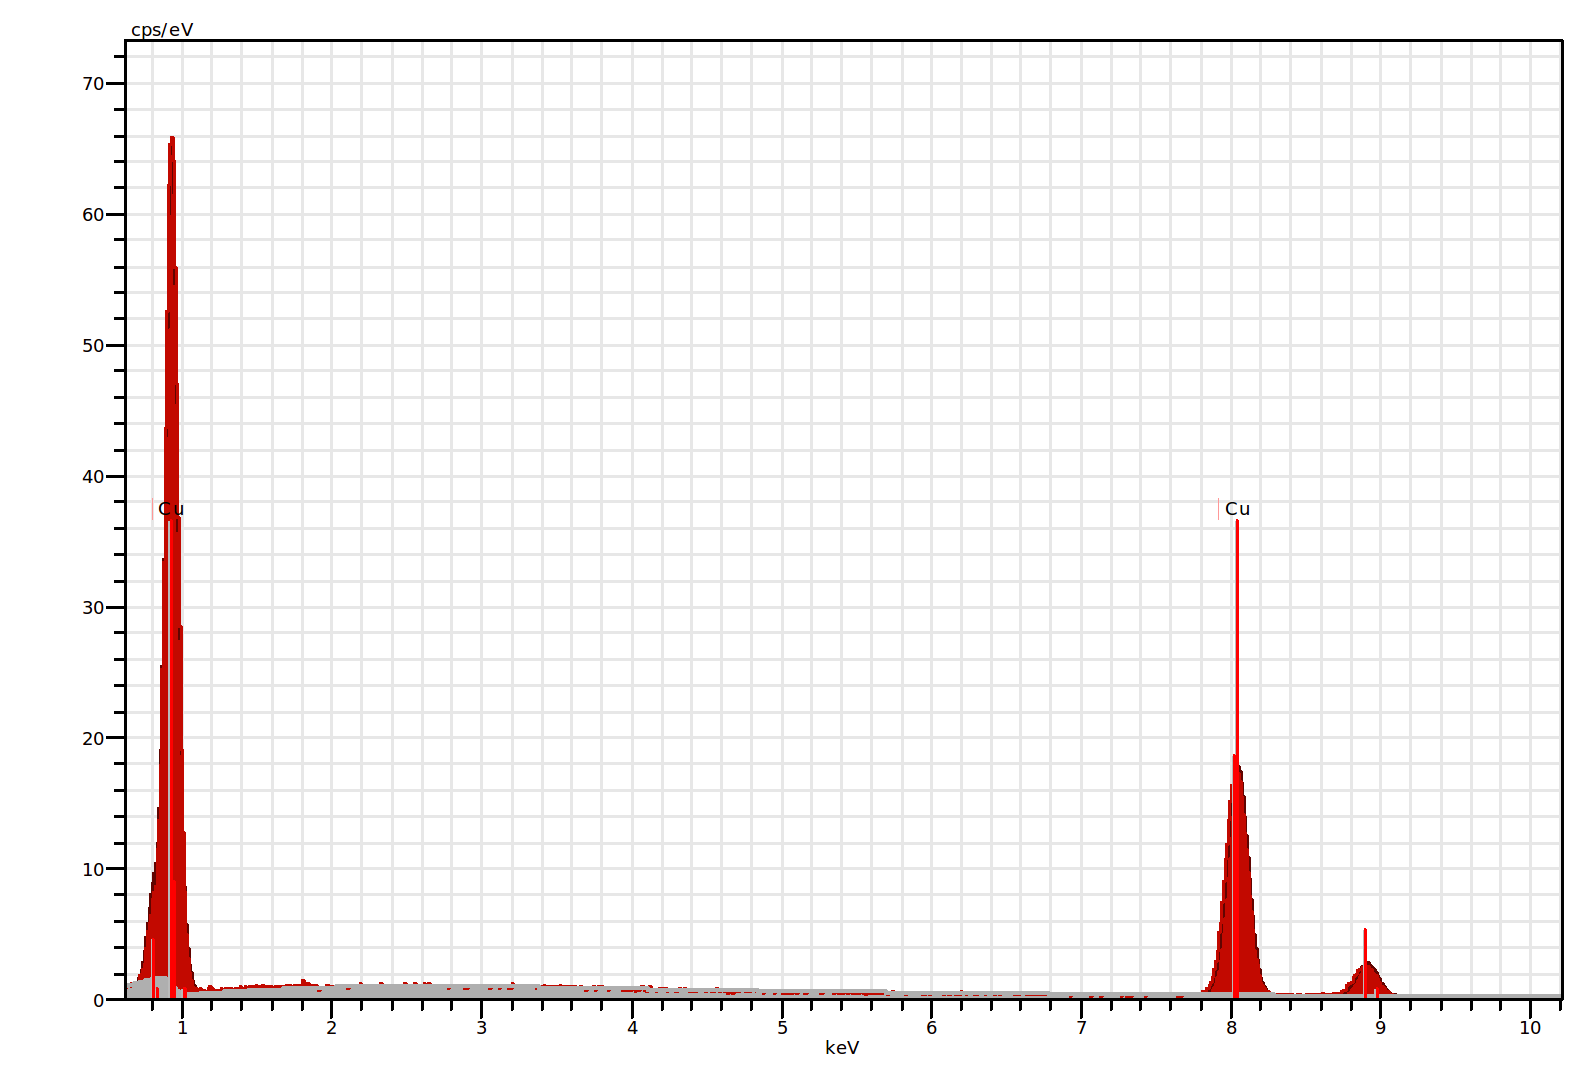
\includegraphics[width=12cm]{graficos/3/Xsp.png}
\caption{Spektrum vzorku 3 v místě X}
\label{o:vz3_X}
\end{figure}


\begin{tabulka}[htbp]
\centering
\begin{BVerbatim}
Spectrum: Ti_Gl_1 16

Element  Series   unn. C norm. C Atom. C Error
                 [wt.-%] [wt.-%] [at.-%]   [%]
----------------------------------------------
Copper  K-series   66,32   74,57   75,11   1,8
Zinc    K-series   22,61   25,43   24,89   0,7
----------------------------------------------
          Total:   88,93  100,00  100,00
\end{BVerbatim}
\caption{Chemické složení vzorku 3 v místě Y}
\label{t:vz03_Y}
\end{tabulka}

\begin{figure}[htbp]
\centering
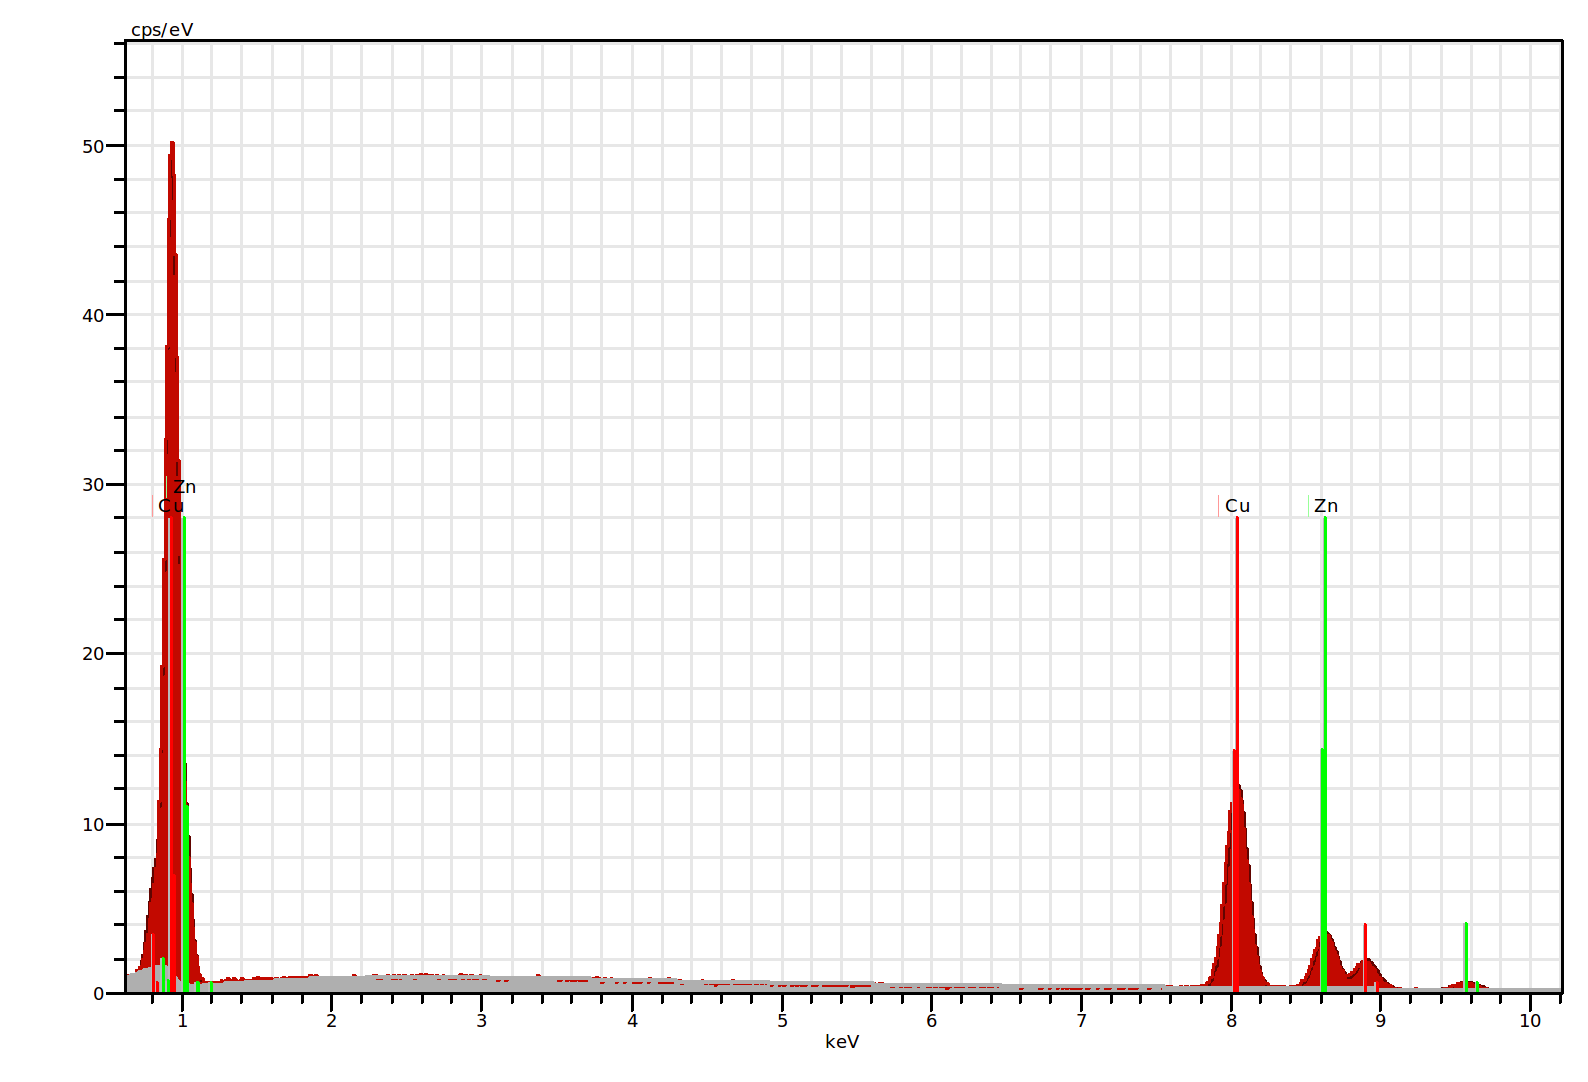
\includegraphics[width=12cm]{graficos/3/Ysp.png}
\caption{Spektrum vzorku 3 v místě Y}
\label{o:vz3_Y}
\end{figure}

\begin{tabulka}[htbp]
\centering
\begin{BVerbatim}
Spectrum: Ti_Gl_1 17

Element  Series   unn. C norm. C Atom. C Error
                 [wt.-%] [wt.-%] [at.-%]   [%]
----------------------------------------------
Iron    K-series   87,76   94,54   95,17   2,4
Copper  K-series    5,07    5,46    4,83   0,2
----------------------------------------------
          Total:   92,82  100,00  100,00
\end{BVerbatim}
\caption{Chemické složení vzorku 3 v místě Z}
\label{t:vz03_Z}
\end{tabulka}

\begin{figure}[htbp]
\centering
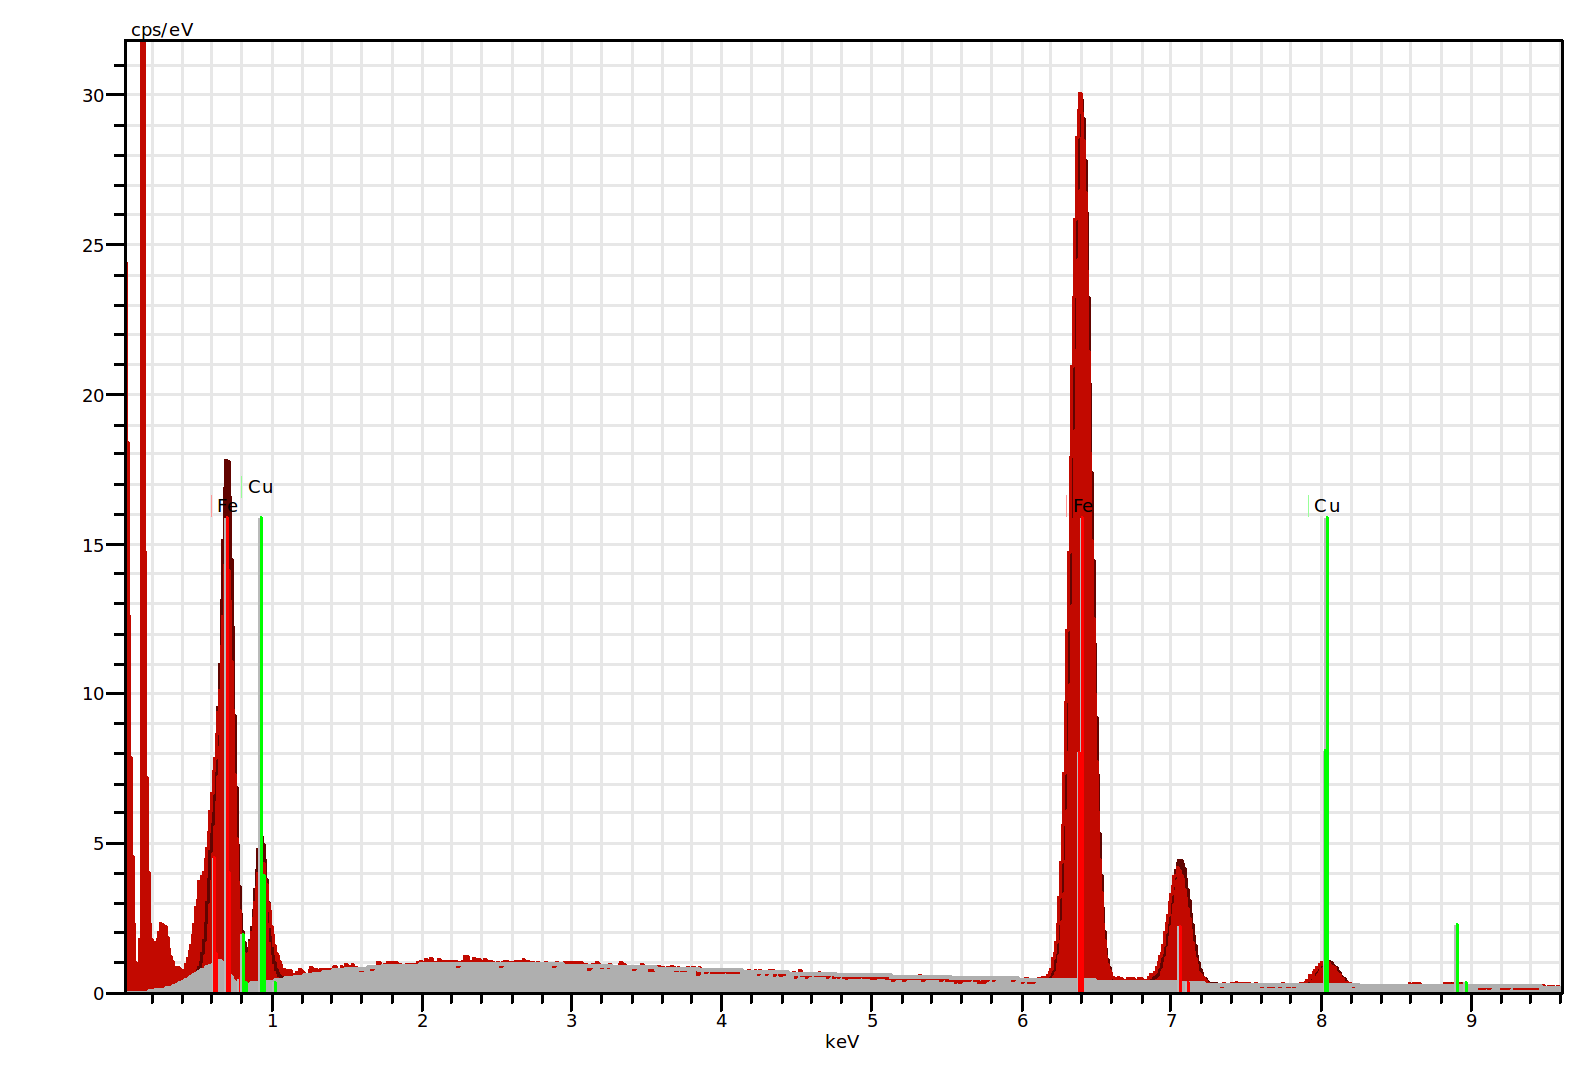
\includegraphics[width=12cm]{graficos/3/Zsp.png}
\caption{Spektrum vzorku 3 v místě Z}
\label{o:vz3_Z}
\end{figure}

\begin{figure}[htbp]
\centering
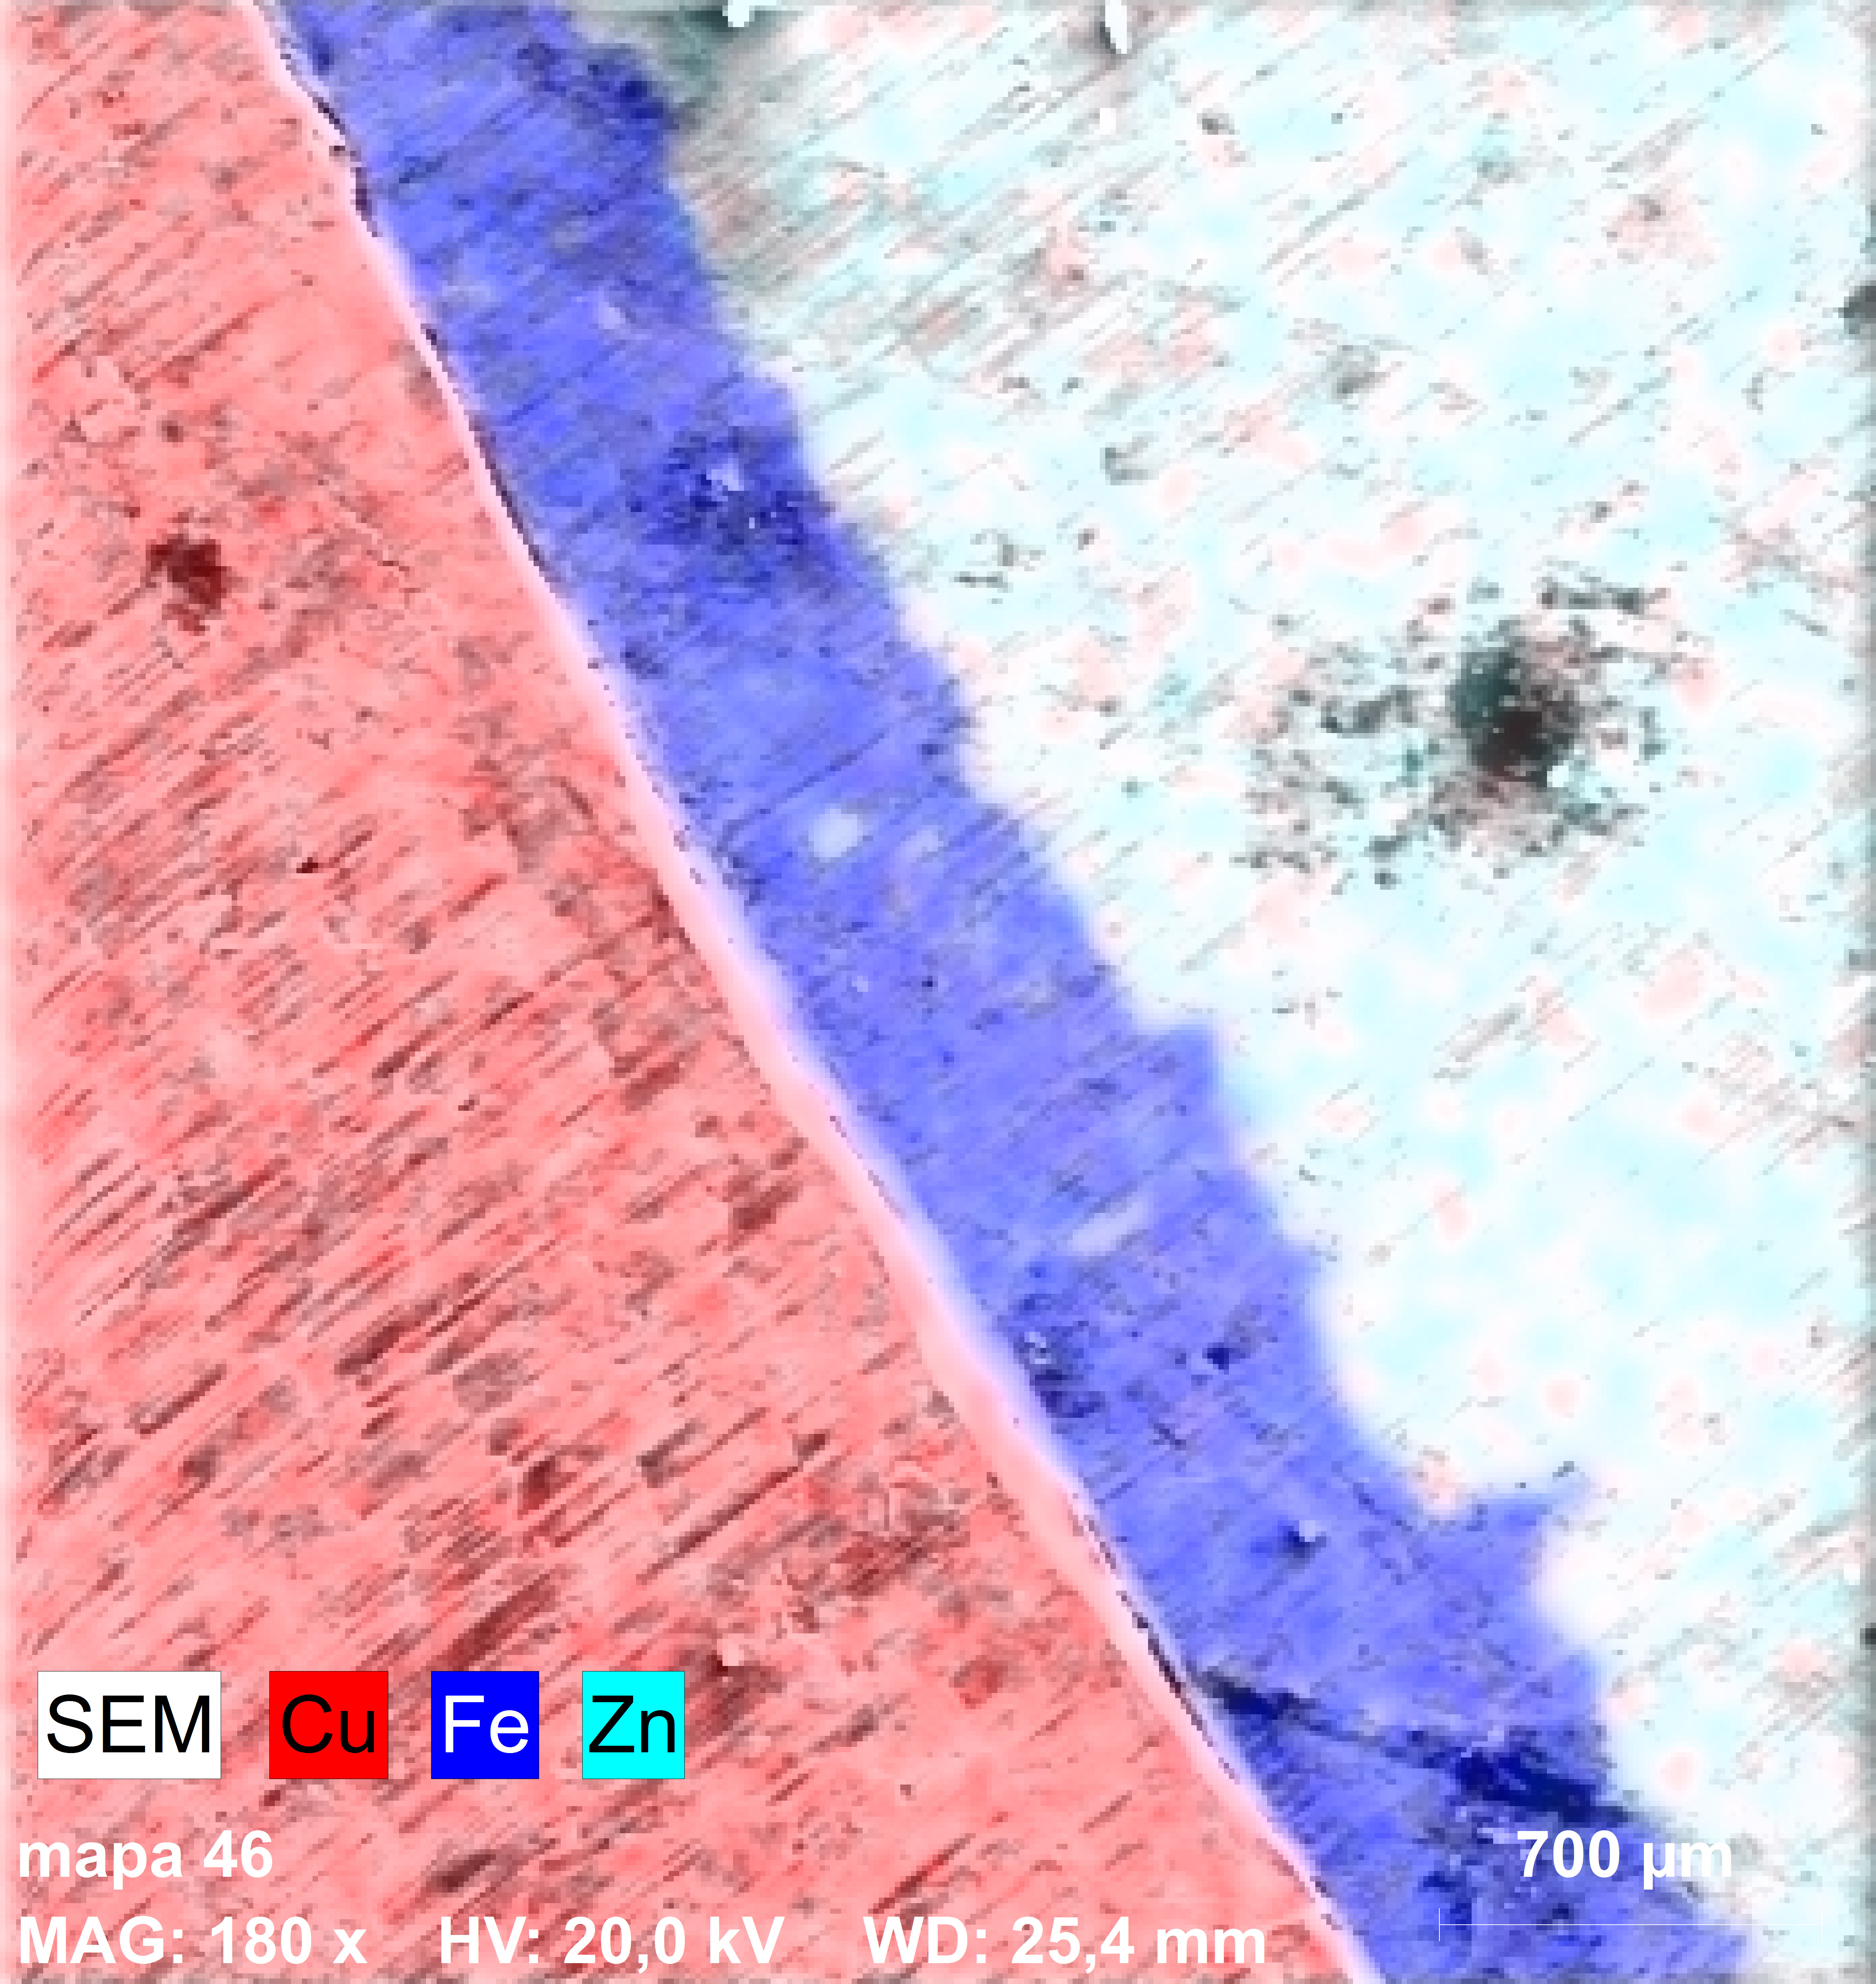
\includegraphics[width=8cm]{graficos/3/2D.png}
\caption{2D sken vzorku 3}
\label{o:vz3_2D}
\end{figure}